\chapter{Controller description} 
\label{cha:description}

This chapter contains a description of the baseline controller, the additional features, the parameters, the dynamic inputs and outputs, and the monitors. The first version of the controller \cite{Hansen13} was a further development of a previous controller used at DTU Wind Energy with new developments inspired by Bossanyi's controller for the 5MW NREL reference turbine \cite{Bossanyi09}. Especially the power error feedback in the pitch controller that keeps the pitch at its minimum below rated power operation represented the most significant change. The current release of the Basic DTU Wind Energy Controller consist of a restructuring of the source code itself and includes the following new features: 
\begin{itemize}
  \item{new optional partial load strategy for optimal tip-speed ratio tracking}
	\item{exclusion zone on the rotor speed} 
	\item{active tower damping by pitch feedback from tower top acceleration} 
	\item{smooth power down for operation in storm conditions} 
	\item{de-rating functionalities [please add Mahmood]}
\end{itemize}
Note that the controller is only considering low speed shaft (LSS) measures of rotational speeds and torques, i.e., there is no gearbox on the drivetrain. The controller can still be used for turbines with a gearbox, when the user transforms torques and speeds between the LSS and high-speed shaft (HSS) using the gear ratio (cf. Table~\ref{t:par2}).

\section{Baseline speed and power control}

The diagram of the baseline controller without the additional functionalities is shown in Figure~\ref{f:diagram}. Note that $k$ denotes the current time step. The controller is switching between the partial and full load operation using the mean pitch angle. These two regions of operation are now described before the switching is explained. The functions $f_1$, $f_2$, and $f_n$ in the diagram are discrete filters described and tested in Appendix~\ref{ch:filters}. The functions $\sigma\in[0:1]$ and $\sigma_h\in[0:1]$ are algebraic functions used for different switching and interpolation operations.

\subsection{Partial load operation}

Two different strategies are implemented for optimal $C_P$ tracking in partial load operation where the PID torque controller is regulating the generator speed. The original strategy is based on a balance between generator and aerodynamic torques to obtain a close to optimal tip speed ratio, and the speed set-point for the PID torque controller is either the minimal or rated generator speed. The new strategy is based on tracking the optimal tip-speed-ratio by varying the generator speed set-point (between its minimum and rated values) according to a first order low-pass filtered wind speed (obtainable from the nacelle anemometers). 

The diagram in Figure~\ref{f:diagram} shows the original routes for the original strategy. The torque reference $Q_{ref,k}$ at the current step $k$ is computed from the LSS generator speed as $K \Omega_k^2 - K_{dot} \dot{\bar \Omega}_k$, where the second term is a inertia reduction component proportional to the time derivative a second order low-pass filtered speed $\dot{\bar \Omega}_k$. This feedback is enforced by setting the torque limits for the PID controller to $Q_{g,min,k}=Q_{g,max,k}=K\Omega_k^2 - K_{dot} \dot{\bar \Omega}_k$ whenever the rotational speed $\Omega_k$ is not close to the minimum speed $\Omega_{min}$, or the rated speed $\Omega_0$. When the rotational speed is close to its bounds, these torque limits will open according to the interpolation factors $\sigma_{min,k}$ and $\sigma_{max,k}$. The torque reference will then be given by the PID controller based on the speed error $e_{Q,k}=\bar\Omega_k -\Omega_{set,k}$, where the set-point is the minimum or rated speed for the original partial load strategy, or can take intermediate values in the new strategy according to the low-pass filtered wind speed as $\bar V_k \lambda_{opt}/R$, where $\lambda_{opt}$ is the optimal tip-speed ratio and $R$ is the outer rotor radius. 

The first order low-pass filtered nacelle wind speed $\bar V_k$ is also used for optimizing the aerodynamic torque through adjustment of the minimum pitch to according to a tabled function $\theta_{min,k}=\theta_{min}(\bar V_k)$ which is provided by the user. Note that the pitch reference is kept at this minimum pitch angle due to the negative power error feedback to the pitch PID controller in the partial load region.

\begin{sidewaysfigure}
\centerline{\epsfig{figure=discrete_diagram.eps,width=1.05\textheight} }
\caption{Diagram of the discrete controller. Note that $k$ denotes the current time step. \label{f:diagram}}
\end{sidewaysfigure}

The interpolation factors for the opening of the torque limits are based on how close the second order low-pass filtered generator speed is from its minimum and rated speeds. The limits can be opened gradually over an interval as described by the function $\sigma$:
\begin{equation}\label{e:sigma_if}
\sigma\left(x_0,x_1;x\right) = \left\{
\begin{array}{rl}
0 & x < x_0 \\
\frac{x - x_0}{x_1 - x_0} & x_0 \le x \ge x_1 \\
1 & x > x_1
\end{array} \right.
\end{equation}
Figure~\ref{f:sigma} shows an example of the $\sigma$-function where $x_0=1$ and $x_1=2$. The parameters for this function used for the interpolation factors $\sigma_{min,k}$ and $\sigma_{max,k}$ are defined as
\begin{align}
\nonumber
\Omega_{min_1} &= \Omega_{min} \\
\nonumber
\Omega_{min_2} &= \Omega_{min}/\gamma \\
\label{e:percentage}
\Omega_{max_1} &= \left(2 \gamma - 1 \right) \Omega_0 \\
\nonumber
\Omega_{max_2} &= \gamma \Omega_0
\end{align}
where $\gamma$ is defined by the user (cf. Table~\ref{t:par}). 

Figure~\ref{f:torque_limits} shows the torque limits in partial load operation of the DTU 10~MW RWT, where the minimum speed is 6~rpm, the rated speed is 9.6~rpm, and the percentage is set to 95~\%. The generator torque limits are closed approximately 6~\% above the minimum speed $\Omega_{min}$ and start opening again at 90~\% and are fully open at 95~\% of the rated speed. When the additional functionality of the generator speed exclusion zone is active then there will also be an opening of the torque limits around this zone (cf. Section~\ref{s:EZ}).

\begin{figure}[t]
\centerline{\epsfig{figure=sigma.eps,width=0.45\textheight} }
\caption{Example of the $\sigma$-function \eqref{e:sigma_if} where $x_0=1$ and $x_1=2$. \label{f:sigma}}
\end{figure}

\begin{figure}[t]
\centerline{
\epsfig{figure=torque_limits_rsa.eps,width=0.8\textwidth} }
\caption{Torque limits in partial load operation of the DTU 10~MW RWT, where the minimum speed is 6~rpm and rated speed is 9.6~rpm. The limits are set to be closed approximately 6~\% above the minimum speed and start opening again at 90~\% and are fully open at 95~\% of the rated speed. \label{f:torque_limits}}
\end{figure}

\subsection{Full load operation}

In full load operation, the torque limits are closed around the torque given by the selected power control strategy. It can be constant power $P_0/\Omega_k$ or constant torque $P_0/\Omega_0$, where $P_0$ is the rated power. In the new version, the user can specify any intermediate strategy where the toque limits in full load operation are set to
\begin{equation}
Q_{g,ref,k}^{full} = \left(1-\alpha_g \right) P_0/\Omega_0 +  \alpha_g P_0/\Omega_k
\end{equation}
where $\alpha_g$ is the user-defined ratio between the constant power ($\alpha_g = 1$) and constant torque ($\alpha_g = 0$) strategy. Note that the unfiltered measured LSS generator speed $\Omega_k$ is used for computation of this reference torque.

The pitch reference angle is obtained from a combined PI feedback of the generator speed and power errors, and a possible differential feedback of the speed error. The speed error is obtained as the difference between the second order low-pass filtered LSS generator speed and the rated speed. The power error is the difference between the measured electrical power $P_k$ and the rated power $P_0$. Both errors are notch filtered around the frequency specified by the user as the free-free drivetrain frequency. This frequency is assumed to be constant although HAWCStab2 eigenvalue analysis often show a small variation with operational point (wind speed). Note that both errors contribute to the same proportional term ($\theta_{P,k}$) and same integral term ($\theta_{I,k}$). The latter is important because it ensures that the reference pitch angle is kept at the minimum pitch angle until rated power is reached; assuming that the right weighting between the integral speed error gain $k_{I,0}$ and power error gain $k_I^P$ has been selected by the user.

The anti-windup is performed such that the controller will react quickly with increased pitch angle if the electrical power suddenly increased above the rated power level. In each time step, the minimum pitch limit is enforced on the reference pitch which is the sum of the proportional, differential, and integral terms $\theta_{ref,k}=\max\left(\theta_{min,k},\theta_{P,k}+\theta_{D,k}+\theta_{I,k}\right)$. The value of the integral term to be used for the integration in the next time step is then recalculated as $\theta_{I,k}=\theta_{ref,k}-\theta_{P,k}-\theta_{D,k}$, which only makes a change to the integral term if the reference pitch is on the minimum limit $\theta_{ref,k}=\theta_{min,k}$. Below rated power, where the proportional term is negative because the rotational speed error is kept close to zero by the torque PID controller, the integral term will therefore be positive. If the electrical power is increased and becomes close to rated power (due to the reaction of the torque PID controller to an increased wind speed), then the proportional term will come close to zero whereas the integral will still be positive and the resulting pitch reference angle will be positive, whereby large power and speed variations are avoided. Note that the same anti-windup scheme is used in the torque PID controller.

The first order low-pass filtered mean of the blade pitch angles $\bar \theta_{m,k}$ is used for scheduling of the gains of the pitch PID controller. A quadratic dependency of the aerodynamic torque gain with collective pitch angle is assumed as
\begin{equation}\label{e:gainsch}
\frac{\partial Q_A}{\partial \theta}= \left. \frac{\partial Q_A}{\partial \theta}\right|_{\theta=0}\left(1 + \frac{\theta}{K_{1}} + \frac{\theta^2}{K_{2}}\right)
\end{equation}
where $Q_A$ denotes the aerodynamic torque, $\theta$ is the collective pitch angle, and $\left. \frac{\partial Q_A}{\partial \theta}\right|_{\theta=0}$ is the aerodynamic gain at zero pitch. The parameters of this expression $K_1$ and $K_2$ can be obtained from curve fitting to the derivative of the aerodynamic torque with respect to collective pitch angle assuming quasi-steady aerodynamics and \emph{frozen wake} (constant induced velocities) as
\begin{equation}\label{e:dqadt}
\frac{\partial Q_A}{\partial \theta} = \frac12 \rho B \int_0^R c(r) U(r)^2 \left(
  C_L'(\alpha(r)) \sin \varphi(r)
- C_D'(\alpha(r)) \cos \varphi(r) \right) r dr
\end{equation}
where $B$ is the number of blades, $R$ is the outer radius of the rotor, $c(r)$ is the radial chord distribution, $U(r)$ is the mean steady state relative inflow velocity along the blade, $C_L'$ and $C_D'$ are the gradients of the lift and drag coefficient curves evaluated at the mean steady state angle of attack $\alpha(r)$ along the blade, and $\varphi(r)$ is the spanwise distribution of inflow angles relative to the rotor plane.

An additional term of the gain-scheduling can be activated to take into account the variation of the aerodynamic damping. A quadratic dependency is assumed also in this case
\begin{equation}\label{e:gainsch_omega}
\frac{\partial Q_A}{\partial \Omega}= \left. \frac{\partial Q_A}{\partial \Omega}\right|_{\theta=0}\left(1 + \frac{\theta}{K_{\Omega\,1}} + \frac{\theta^2}{K_{\Omega\,2}}\right)
\end{equation}
A detailed description of this scheme is described by Tibaldi~et~al.~\cite{tibaldi_effects_2014}.

Figure~\ref{f:gainsch} shows the aerodynamic torque gradients obtained from HAWCStab2 for the DTU 10~MW RWT together with the fit of the quadratic expressions \eqref{e:gainsch} and \eqref{e:gainsch_omega}. The fitted parameters are shown as inputs number 21, 22, 51, and 52 in Table~\ref{t:par} of Section~\ref{s:par}. Often, a linear fit is sufficient and it is assumed when the user enters $K_2=0$ (note that $K_1$ then is the angle where the aerodynamic gain is doubled). The gain scheduling factor based on the filtered mean pitch angle $\eta_{A,k}$ is the inverse of the expression in the parenthesis of \eqref{e:gainsch}. A nonlinear gain factor $\eta_{nl,k}$ based on the generator speed error is also added for increased sensitivity of the pitch PID controller by large speed excursions.


\begin{figure}[!t]
\begin{center}
\parbox{0.45\columnwidth}{\mbox{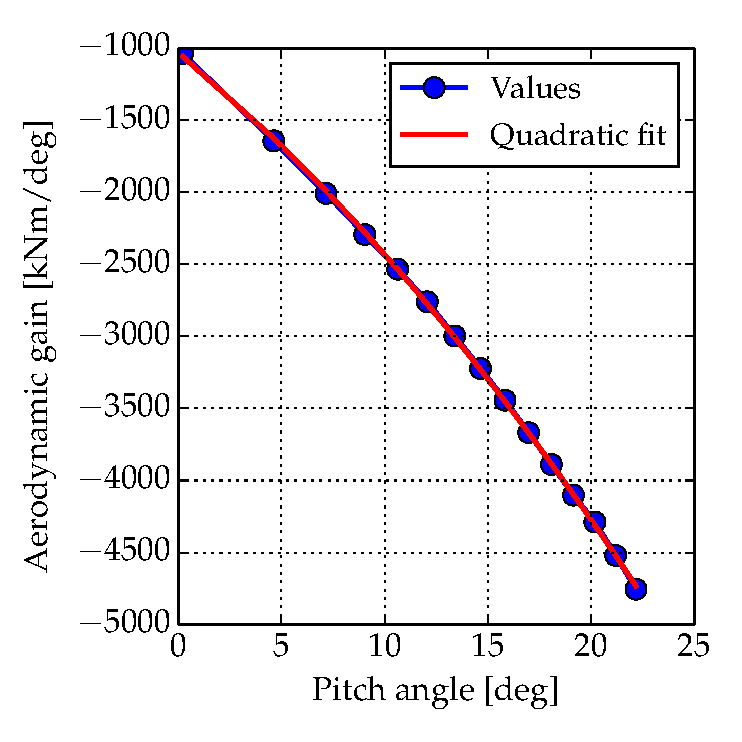
\includegraphics[keepaspectratio=true,width=0.45\columnwidth]{AG}}\center{\textit{a) Aerodynamic gainl}}}\quad
\parbox{0.5\columnwidth}{\mbox{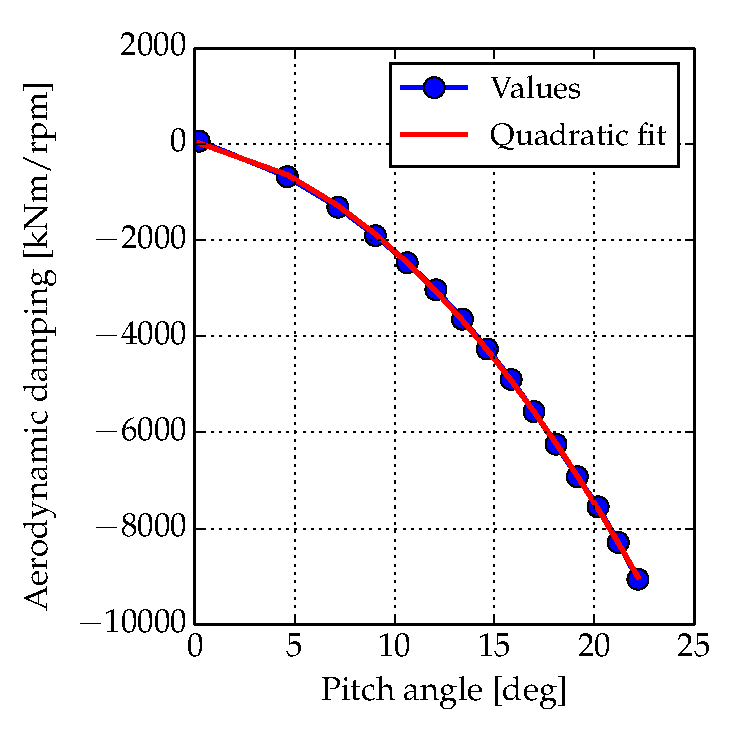
\includegraphics[keepaspectratio=true,width=0.45\columnwidth]{AD}}\center{\textit{b) Aerodynamic damping}}}
\caption{Aerodynamic gain and aerodynamic damping for the DTU 10~MW RWT. Queasi-steady values computed with HAWCStab2 and quadratic fitting.}\label{f:gainsch}
\end{center}
\end{figure}

\subsection{Switching between partial and full load operation}

The switching between partial and full load operation of the torque controller is based on interpolating between the torque limits of partial and full load operation. The interpolation factor $\sigma_{\theta,k}$ is computed from the unfiltered mean pitch angle $\theta_{m,k}$ using the special switching function $\sigma_h \left(\theta_{f}; \bar \theta_{m,k} , \theta_{min,k}\right)$ plotted in Figure~\ref{f:sigma_hys}. The interpolation factor linearly increases to one as the mean pitch angle increases from the current minimum pitch angle $\theta_{min,k}$ to the angle $\theta_{min,k} + \theta_{f}$, where $\theta_f$ is a user-defined full load angle. Once the mean pitch angle has been above $\theta_{min,k} + \theta_{f}$, a hysteresis feature ensures that the interpolation factor will remain one (full load operation) until the mean pitch angle becomes lower than the current minimum pitch angle $\theta_{min,k}$ plus 0.01~deg.

\begin{figure}[t]
\centerline{\epsfig{figure=sigma_hys.eps,width=0.45\textheight} }
\caption{Example of the special switching function $\sigma_h \left(\theta_{f}; \bar \theta_{m,k} , \theta_{min,k}\right)$ that includes a hysteresis meaning that the interpolation factor will remain 1 once the mean pitch angle was the user-defined parameter $\theta_{f}$ (here equal 2~deg) above the current minimum pitch angle (here equal 0~deg). \label{f:sigma_hys}}
\end{figure}




%%%%%%%%%%%%%%%%%%%%%%%%%%%%%%%%%%%%%%%%%%%%%%%%%%%%%%%%%%%

\section{Additional functionalities}

Additional functionalities are implemented on top of the baseline speed and power control which are described in this section.

\subsection{Additional nonlinear pitch control term}

A pitch rate can be added to the reference pitch angle from the pitch controller during extreme event where severe over-speed can occur. The added pitch rate is computed from the filtered speed error and the time derivative of the filtered generator speed:
\begin{align}
	\dot{\theta}_{+} &= \dot{\theta}_{+} + k_{os} ( \dot{\bar{\Omega}}_k/\Omega_{os} + e_{\Omega,k}/\dot{\Omega}_{os} ) &\text{ for } ( \dot{\bar{\Omega}}_k/\Omega_{os} + e_{\Omega,k}/\dot{\Omega}_{os} ) > 1 \\
	\dot{\theta}_{+} &= \dot{\theta}_{+} &\text{ for } ( \dot{\bar{\Omega}}_k/\Omega_{os} + e_{\Omega,k}/\dot{\Omega}_{os} ) \leq 1	
\end{align}
This control block is only active if the corresponding input parameters are all non-zero ($\Omega_{os}$,$\dot{\Omega}_{os}$,$k_{os}$) $\neq$ 0.

\subsection{Active dampers (code and text should be revised)}

Two dampers are part of the controller, one to reduce drivetrain vibrations and one to reduce longitudinal tower vibrations. The dampers have the same structure. They are formed as a series of a bandpass filter, a notch filter, and a time delay. The bandpass filter isolates the desired frequency to damp. The notch filter further reduces the component of the signal at the frequency of a mode that could be excited by the damper. The time delay compensates the phase shift due to the signal processing and system phase lag.
The filtered signal is then multiplied by a factor to scale the damping effects.

\subsubsection{Drivetrain damper}
\label{s:dmp}

The drivetrain damper receives as input the unfiltered measured generator LSS speed $\Omega_k$. The band-pass filter has the center frequency equals to the free-free drivetrain torsional frequency $\omega_{dt}$. The notch filter has center frequency of $\omega_{n,dtd}$. The filtered speed $\Omega_{d,k}$ is multiplied by a gain factor $k_{dmp}$ and added to the torque feedback from the PID controller to give the generator torque reference. Note that this drivetrain damper is always active when $k_{dmp}\ne0$. 

The performance of drivetrain damper can bee seen from Figure~\ref{f:DT_damper}, where the vibration of the drivetrain mode are actively reduced by the damper.

\subsubsection{Longitudinal tower damper}
\label{s:TTdmp}


The measured tower top longitudinal acceleration $a_{TT}$ is used as input to the longitudinal tower damper. The band-pass filter has the center frequency equals to the longitudinal tower mode frequency $\omega_{bp,td}$ and damping $\zeta_{bp,td}$. The notch filter has center frequency of  $\omega_{n,td}$ and damping $\zeta_{n,td}$. The gain of the tower damper is defined as $k_{td}$. 

The performance of the longitudinal tower damper can bee seen from Figure~\ref{f:TT_damper}, where the vibration of the first longitudinal tower mode are actively reduced.

\subsection{Exclusion zone (text should be revised)}
\label{s:EZ}

The exclusion zone functionality can be used to avoid resonant conditions between the 3P excitation and the first lateral tower mode. The functionality logic is based on a finite-state machine with diagram presented in Figure~\ref{f:EZ_SD}. States 0 and 3 are variable rotor speed regimes below the exclusion zone minimal speed and above the exclusion zone maximal speed, respectively. States 1 and 2 are constant rotor speed regimes, where the speed is stabilized on $\Omega_L$ or $\Omega_H$ by appropriate switching of the reference speed of the generator torque PID controller. During transients from state 1 to state 2 and the other way around, the reference speed switch is low-pass filtered with a first-order filter with time constant $\tau_{EZ}$. The torque dependency on rotor speed can be seen from Figure~\ref{f:EZ_torque}. Finally, the exclusion zone functionality can be seen from Figure~\ref{f:EZ}, where the rotor speed, tower top fore-aft and side to side acceleration is displayed for active and deactivated exclusion zone.

Figure~\ref{f:EZ_torque_limits} shows the torque limits when the exclusion zone functionality is active. The torque limits starts to open at 99~\% of the exclusion zone minimal speed $\Omega_{L}$ and are closed  1~\% above the exclusion zone maximal speed $\Omega_{H}$. Where the spline function is used to guarantee smooth transient. The maximal torque limit is set to $Q_{g,max}$ 5~\% above the $Q_{g_{\Omega_{L}}}$ and the minimal torque is set to $Q_{g,min}$ 95~\% of the $Q_{g_{\Omega_{H}}}$.

\begin{figure}[b!]
\centerline{
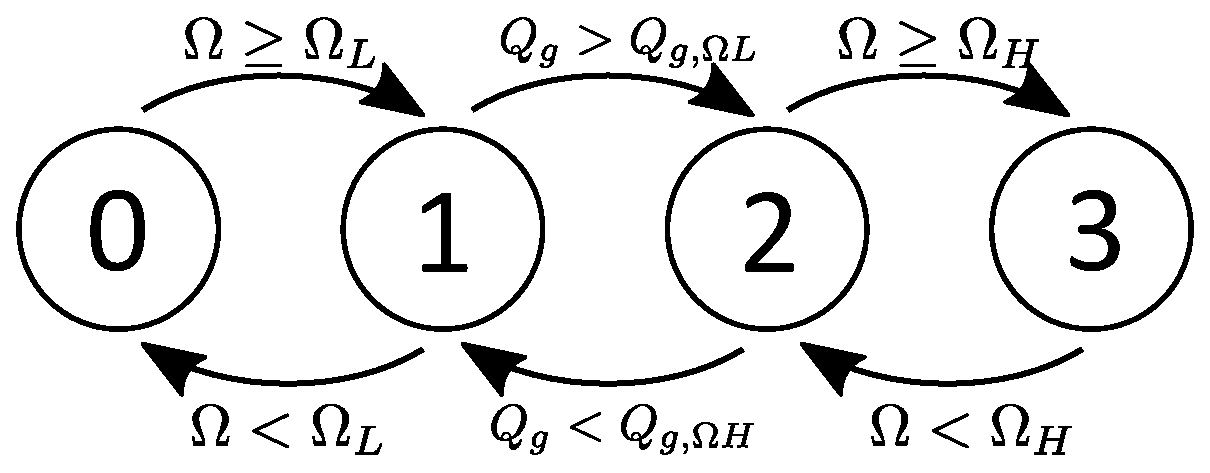
\includegraphics[width=0.4\textwidth]{ExclZone_state_diagram.eps} }
\caption{Exclusion zone logic diagram. \label{f:EZ_SD}}
\end{figure}

\begin{figure}[tb]
\centerline{
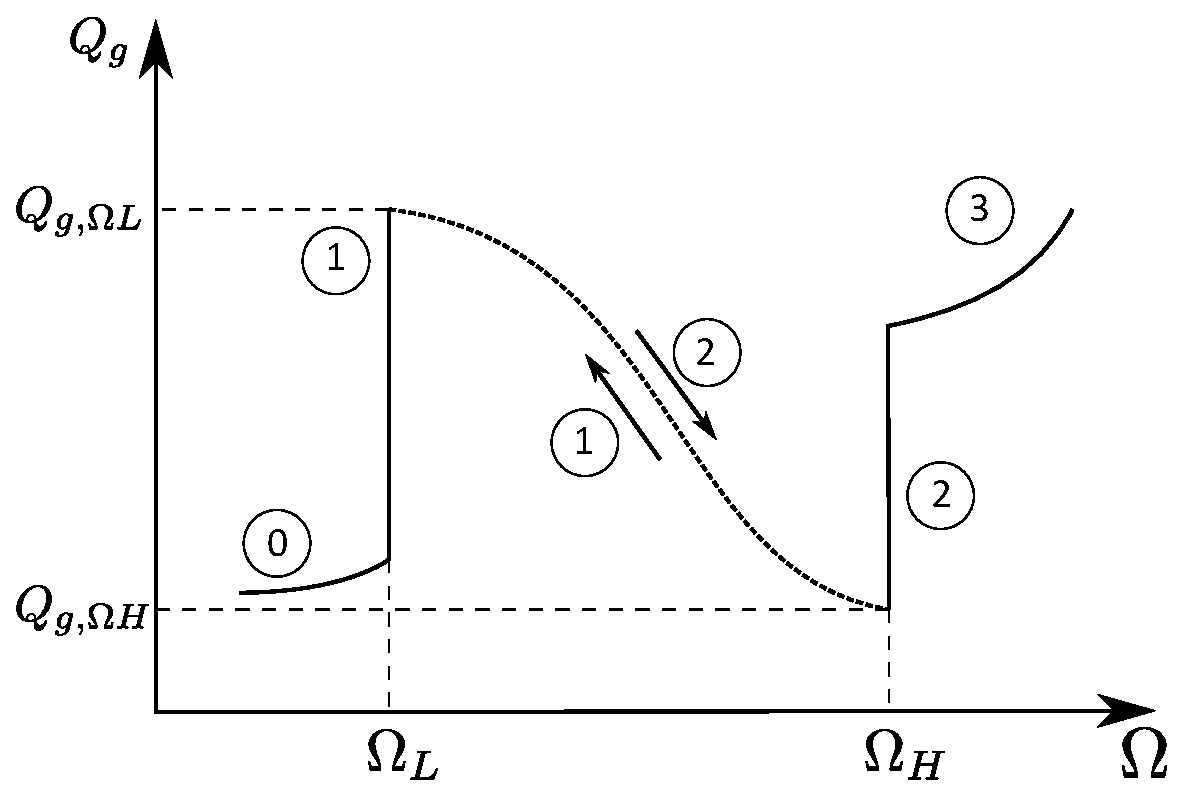
\includegraphics[width=0.6\textwidth]{ExclZone_torque.eps} }
\caption{Exclusion zone torque curve. \label{f:EZ_torque}}
\end{figure}

\begin{figure}[tb]
\centerline{
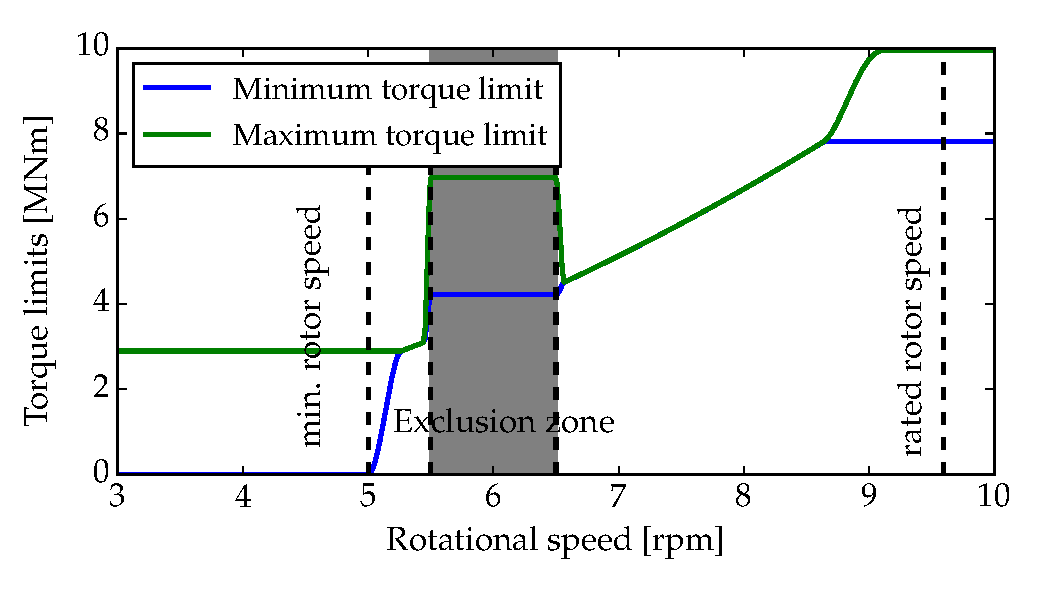
\includegraphics[width=0.7\textwidth]{torque_limits_rsa_exclusionzone.eps} }
\caption{Torque limits in partial load operation of the DTU 10~MW RWT when the rotor speed exclusion zone is active (note that the minimum rotational speed is lowered to 5~rpm compared to the 6~rpm in Figure~\ref{f:torque_limits}). \label{f:EZ_torque_limits}}
\end{figure}


\subsection{Storm control (redundant with new curtailment features?)}

The controller includes also a feature for regulation above the standard cut-out wind speed, i.e. in storm conditions. The reference rotational speed $\Omega_{set, k}$ used for the pitch regulation is linearly reduced, based on a low-pass filtered measurement of the wind speed. The reduction goes from the rated rotational speed value ($\Omega_0$) at the standard cut-out wind speed, now defined as storm wind speed ($V_{storm}$), to the minimum allowed rotor speed value ($\Omega_{min}$) at a new cut-out wind speed ($V_{cut-out}$). The generator torque is kept at its rated value.

%%%%%%%%%%%%%%%%%%%%%%%%%%%%%%%%%%%%%%%%%%%%%%%%%%%%%%%%%%%%%%%%%%%%%%%%%%%%%%
\clearpage

\section{Parameters}
\label{s:par}

All parameters of the controller are transferred to the DLL using HAWC2 commands for the \verb|init_regulation| routine of the type2 DLL \cite{Larsen12}. Details of all 52 parameters are given in Table~\ref{t:par}, where the notation of the parameters used in the diagram of Figure~\ref{f:diagram} and some additional notations can also be seen. Additional features can be enabled by using the \verb|init_regulation_advanced| instead, this routine requires 75 parameters, where the first 52 are identical to those of \verb|init_regulation|. The additional parameters can be found in Table~\ref{t:par2}. If any of these parameters are set to zero they are not read and their default value will be used. If all parameters of a particular feature are zero then this feature is inactive, except for the drivetrain damper which will be active if the input parameters 10 and 38 are non-zero.

\begin{table}[t]
\begin{center}
\begin{tabular}{r|c|p{11.5cm}}
Input &  & Additional explanation \\ \hline
1 & $P_0$   			& Rated power [kW]\\
2 & $\Omega_{min}$& Minimum rotor (LSS) speed [rad/s]\\
3 & $\Omega_0$ 		& Rated rotor (LSS) speed [rad/s] \\
4 & -     				& Maximum allowable generator torque [Nm]. An upper limit set on the torque reference signal. \\
5 & $\theta_{min}$& Minimum pitch angle [deg] if this input is less than 90~deg. Otherwise, the init routine will search for a file with the name ``wptable.n'', where ``n'' is a character string obtained from the integer value of the input. In the shown example, this file is therefore ``wptable.100''. The file format is first line contains an integer with the number of subsequent lines, which contain two numbers each, wind speed and minimum pitch angle in degrees. An example is shown in Table~\ref{t:wptable}.\\
6 & $\theta_{max}$	& Maximum pitch angle [deg] \\
7 & - 				& Maximum pitch velocity operation [deg/s]. An upper limit set on the rate of change of the pitch reference signal\\
\hline
8 & $\omega_{\Omega}$ 	& Frequency of generator speed filter [Hz] \\
9 & $\zeta_{\Omega}$ 	& Damping ratio of speed filter [-] \\
10 & $\omega_{dt}$ 		& Frequency of free-free DT torsion mode [Hz], used for a notch filter and a band-pass filter of the damper. \\
\hline
11 & $K$ 			  & Optimal $C_P$ tracking factor [Nm/(rad/s)$^2$], $K=\eta \frac12 \rho A C_{P,opt} R^3/\lambda_{opt}^3$. If $K\le0$ then the optimal tip-speed ratio tracking strategy in partial load operation is used.\\
12 & $k_P^g$ 		& Proportional gain of torque controller [Nm/(rad/s)] \\
13 & $k_I^g$ 		& Integral gain of torque controller [Nm/rad] \\
14 & $k_D^g$ 		& Differential gain of torque controller [Nm/(rad/s$^2$)] \\
15 & - 			    & Generator control switch [1=constant power, 0=constant torque, or interpolation between the two] \\
16 & $k_{P0}$ 	& Proportional gain of pitch controller [rad/(rad/s)] \\
17 & $k_{I}$ 		& Integral gain of pitch controller [rad/rad]\\
18 & $k_{D}$ 		& Differential gain of pitch controller [rad/(rad/s$^2$)] \\
19 & $k_P^P$ 		& Proportional power error gain [rad/W] \\
20 & $k_I^P$ 		& Integral power error gain [rad/(Ws)] \\
21 & $K_1$ 			& Coefficient of linear term in aerodynamic gain scheduling [deg] \\
22 & $K_2$ 			& Coefficient of quadratic term in aerodynamic gain scheduling [deg$^2$]. If $K_2=0$ then linear gain scheduling is assumed. \\
23 & $\Omega_2/\Omega_0$ & Normalized speed where the pitch controller gains are doubled.\\
\hline
24 & - 			& Cut-in time [s], no cut-in is simulated if zero or negative. \\
25 & - 			& A time delay for the cut-in procedure given in the unit [1/1P] corresponding to the rotational period at rated speed.\\
26 & -  		& Shut-down time [s], no shut-down simulated if zero or negative. \\
27 & - 			& Time of linear torque cut-out during a generator assisted stop [s] \\
28 & - 			& Stop type [1=normal, 2=emergency] as described in Section~\ref{s:cutout}. \\
29 & -   		& Time delay for pitch stop after shut-down signal [s] \\
30 & - 			& Maximum pitch velocity during initial period of stop [deg/s] \\
31 & -  		& Time of initial pitch stop phase [s] (maintains pitch speed specified in constant 30).\\
32 & - 			& Maximum pitch velocity during final phase of stop [deg/s]
\end{tabular}
\end{center}
\end{table}

\begin{table}[t!]
\begin{center}
\begin{tabular}{r|c|p{11.5cm}}
Input &  			& Additional explanation \\ \hline
33 & $\tau_{g}$ 	& Time for the maximum torque rate = Maximum allowable generator torque/(constant 33 + 0.01s) [s] \\
34 & $\theta_{f_1}$ 	& Angle above lowest minimum pitch angle for switch to full load [deg] \\
35 & $\gamma$ 		& Percentage of the rated speed when the torque limits are fully opened [\%] \\
36 & $\tau_V \Omega_0 /(2\pi)$ 		& Time constant of 1st order filter on wind speed used for minimum pitch [1/1P] \\
37 & $\tau_{\theta} \Omega_0 /(2\pi)$ & Time constant of 1st order filter on pitch angle for gain scheduling [1/1P] \\
38 & $k_{dtd}$ 		& Proportional gain of DT damper [Nm/(rad/s)], requires frequency in input 10. \\
\hline
39 & - 			& Overspeed percentage before initiating turbine controller alarm (shut-down) [\%]\\
\hline
40 & $\Omega_{os}$ 	& Rotor speed error scaling factor  [rad/s] \\
41 & $\dot{\Omega}_{os}$ & Rotor acceleration error scaling factor  [rad/s${}^2$] \\
42 & $k_{os}$ 		& Pitch rate gain  [rad/s] \\
\hline
43 & 	$V_{storm}$		& Wind speed 'Vstorm' above which derating of rotor speed is used [m/s] \\
44 & 	$V_{cut-out}$	& Cut-out wind speed (only used for derating of rotor speed in storm) [m/s] \\
\hline
45 &  		-		& Overspeed percentage before initiating safety system alarm (shut-down) [\%] \\
46 &  		-		& Maximum low-pass filtered tower top acceleration level before initiating turbine controller alarm (shut-down) [m/s$^2$] \\
\hline
47 &  		$R$		& Rotor radius [m] \\
\hline
48 &  		$K_{dot}$	& Proportional gain on rotor acceleration in variable speed region [Nm/(rad/s${}^2$)] (not used when zero) \\
\hline
49 &  	$\lambda_{opt}$	& Optimal tip speed ratio [-] (only used when constant 11 $K\le0$). \\
\hline
50 &  	$k_{P0,\Omega}$	& Aerodynamic DT damping coefficient at the operational point of zero pitch angle [Nm/(rad/s)] (not used when zero)\\
51 &  	$K_{\Omega 1}$	& Coefficient of linear term in aerodynamic DT damping scheduling, KK1 [deg] \\
52 &	$K_{\Omega 2}$	& Coefficient of quadratic term in aerodynamic DT damping scheduling, KK2 [deg${}^2$] \\
\end{tabular}
\caption{All parameters of the controller related to the parameters shown in the diagram in Figure~\ref{f:diagram} . \label{t:par}}
\end{center}
\end{table}




\begin{table}[t!]
\begin{center}
\begin{tabular}{r|c|p{11.5cm}}
Input &  			& Additional explanation  \\ \hline
 53   &	  $\Omega_L$	    & Exclusion zone: Lower speed limit [rad/s]              (Default 0 used if zero)\\ 
 54   &  $Q_{g\Omega L}$	& Exclusion zone: Generator torque at lower limit [Nm]   (Default 0 used if zero)\\ 
 55   &  $\Omega_H$ 	    & Exclusion zone: Upper speed limit [rad/s] (if $\le 0$ then exclusion zone functionality is inactive)\\ 
 56   &  $Q_{G\Omega H}$& Exclusion zone: Generator torque at upper limit [Nm]     (Default 0 used if zero)\\ 
 57   &	  $\tau_{EZ}$	& Time constant of reference switching at exclusion zone [s] (Default 0 used if zero)\\   
\hline
 58  & $\omega_{n,dtd}$ 	& Frequency of DT damper notch filter [Hz]                  (Default 10$\times$ input 10 used if zero)\\ 
 59  & $\zeta_{bp,dtd}$	& Damping of DT damper BP filter [-]                          (Default 0.02 used if zero)\\ 
 60  & $\zeta_{n,dtd}$	& Damping of DT damper notch filter [-]                       (Default 0.01 used if zero)\\ 
 61  & - 			& Phase lag of DT damper [s] (maximum 40 time steps)                    (Default 0 used if zero) \\ 
\hline
 62  & $\omega_{bp, td}$	& Frequency of tower damper BP filter [Hz]                   (Default 10 used if zero)\\ 
 63  & $\omega_{n, td}$	& Frequency of tower damper notch filter [Hz]                  (Default 10 used if zero)\\ 
 64  & $\zeta_{bp,td}$	& Damping of tower damper  BP filter [-]                       (Default 0.02 used if zero)\\ 
 65  & $\zeta_{n,td}$	  & Damping of tower damper  notch filter [-]                    (Default 0.01 used if zero)\\ 
 66  & $k_{td}$ 		& Gain of tower damper  [-]                                        (Default 0 used if zero)\\ 
 67  & - 			& Phase lag of tower damper  [s] (maximum 40 time steps)                 (Default 0 used if zero)\\ 
 68  & - 			& Time constant of 1st order filter on PWR used for tower damper GS [Hz] (Default 10 used if zero)\\ 
 69  & $\eta_{TT\,L}$ 	& Lower PWR limit used for tower damper smooth activation [-]  (Default 0 used if zero)\\ 
 70  & $\eta_{TT\,U}$  	& Upper PWR limit used for tower damper smooth activation [-]  (Default 0 used if zero) \\ 
\hline
 71  & - 			& Frequency of notch filter of tower lateral mode [Hz]. (Default 100 used if zero)\\ 
 72  & - 			& Damping of notch filter of tower lateral mode [-].    (Default 0.01 used if zero)\\ 
\hline
 73  & - 			& Maximum low-pass filtered tower top acceleration level before initiating safety system alarm (shut-down) [m/s${}^2$]. (Default 1.1$\times$input 46 used if zero) \\ 
 74  & - 			& Time constant of first order filter on tower top acceleration [1/1P] (Default 1 used if zero)\\ 
\hline
 75  & - 			& Parameter for pitch deviation monitoring. The format is 1,nnn,mmm where 'nnn' [s] is the period of the moving average and 'mmm' is threshold of the deviation [0.1 deg] (functionality is inactive if value $<$ 1,000,000) \\ 
 \hline
 76  &- 			& Gear ratio used for the calculation of the LSS rotational speeds and the HSS generator torque reference [-] (Default 1 if zero)\\
\end{tabular}
\caption{All the advanced parameters of the controller related to the exclusion zone, drivetrain damper, tower damper, and additional filters. \label{t:par2}}
\end{center}
\end{table}


\begin{table}[t]
\begin{center}
\begin{verbatim}
7
 0.0 3.0
 4.0 3.0
 5.0 2.5
 6.0 1.7
 7.0 0.8
 8.0 0.0
50.0 0.0
\end{verbatim}
\caption{Example of a ``wptable.n'' file. First line contains an integer with the number of subsequent lines, which contain two numbers each, wind speed and minimum pitch angle in degrees.\label{t:wptable}}
\end{center}
\end{table}

\section{Cut-in procedure - start up at any wind speed}

The blades are initially pitched out to maximum pitch and then at a given time in the simulation (input 24), the start-up procedure is started. First, the low-pass filtered wind speed and the measured rotational speed pitch reference are used to track approximately 6~deg angle of attack at the section of 75~\% blade radius. This pitch angle will therefore decrease as the rotor speeds up. The generator is still cut-out until the rotor speed is sufficient high, where both the torque and pitch controllers become active, unless the speed-up has taken less then the time delay defined in input 25; in such case there will be a soft cut-in of the generator torque. During the initial rotor speed-up, the speed error PID terms of both torque and pitch controllers are active and the set-point of it is the rated rotor speed. The controllers are therefore ready to take over when the speed is high enough. The controller should thereafter be operating normally, and this start-up will take less than 100~s for the DTU 10~MW RWT.

There should be no need for wind ramping for the controller to start up; however, caution should be made on not to start high wind speed (above rated) simulations with too high initial rotational speed. Too high initial rotor speed may cause the pitch and torque controllers to overreact and they may enter a state of competition. If the user can allow long start-up periods then the most stable way is set a late cut-in time to let the rotor slow down to idling before the cut-in starts. However, at low wind speeds, the start-up will then take some time, and a very early cut-in (e.g. 0.1~s) is recommended, combined with an initial rotational speed is set to a value 50-75~\% of the minimum speed.


\section{Shut-down procedures} \label{s:cutout}

The user may specify a time in the simulation for a normal shut-down in input 26, and which time the generator torque reference is linearly decreased to zero using a user-defined time constant (input 27). At the cut-out time plus the first user-defined time delay in input 29, the blades will start to pitch out by setting the reference pitch angle to the maximum pitch angle. The pitching is linear with two different constant speeds, first the pitch velocity specified in input 30, and then after the additional time specified in input 31 the pitch velocity is defined by input 32.

\section{System monitoring}

Two different levels of system monitoring are implemented in the controller. The first level is inside the wind turbine controller and it deals with grid failure, generator overspeed, tower-top acceleration, and reverse generator speed. When one of these monitoring alarms is triggered the wind turbine will shut-down with a normal procedure. The thresholds for the overspeed and the tower-top acceleration can be set in inputs 39 and 46. When using the extra input parameters of \verb|init_regulation_advanced|, the user can also activate a monitoring of the pitch angles to detect a deviation from the reference signal. Input 75 contains two parameters: a time period of a running average and a threshold on the deviation angle; a normal shut-down is commenced if one of the differences between running averages of the actual and reference pitch angles exceeds the threshold.

The second level of monitoring is outside the wind turbine controller and it acts as a safety system overriding all the signals coming from the controller. This system monitors the overspeed and the tower-top acceleration, and if activated, it leads to an emergency stop. The threshold on the safety system overspeed monitor can be set in input 45, whereas the threshold on the tower-top acceleration by default is set to 1.1 times the first level threshold. If the user wants to set a different safety system threshold on the tower accelerations then it is done by input 73.

\clearpage


\section{Operational status} \label{s:status}
The controller operation is divided into different statuses. Each status correspond to a specific conditions. The status of the controller can be seen from the output number 22.
the different statuses are:
\begin{itemize}
\item -2: stand-still.
\item -1: start-up procedure.
\item 0: normal operation.
\item 1: overspeed monitoring. An overspeed has been detected and the turbine will shut-down. Threshold value in input 45.
\item 2: grid failure. A grid failure has been triggered and the turbine will shut-down.
\item 3: tower-top acceleration monitoring. An excessive tower top acceleration has been detected and the turbine will shut-down. Threshold value in input 46.
\item 4: shut-down procedure with normal stop.
\item 5: shut-down procedure with emergency stop.
\item 6: reverse speed. A reverse speed of the generator rotational speed has been detected and the turbine will shut-down.
\item 7: deviation of pitch signals. Input 75 set a running average time and threshold on the largest allowable deviation from the reference.
\end{itemize} 

\section{Dynamic inputs and outputs}

As input during simulations, the controller requires the time [s], the generator LSS speed [rad/s], the pitch angles of three blades [rad], the three components of the wind speed at hub height [m/s] (the first and second of these three components must be the two horizontal components that are used internally to compute the horizontal vector sum), the electrical power [W], the status flag of the grid connection [0/1], and the two horizontal accelerations of the tower top. Table~\ref{t:input} shows the HAWC2 commands that provide these eight controller inputs for the DTU 10~MW RWT. Note that if the rotor only has two blades, then the controller may still be used by repeating a blade pitch angle output to the controller. However, this trick is only valid if there is no additional cycle, or individual pitch controller appended to this controller.

\begin{table}[t]
\center
\begin{verbatim}
general time ; [s]     
constraint bearing1 shaft_rot 1 only 2 ; Drivetrain speed [rad/s]
constraint bearing2 pitch1 1 only 1; [rad]         
constraint bearing2 pitch2 1 only 1; [rad]                               
constraint bearing2 pitch3 1 only 1; [rad]                               
wind free_wind 1 0.0 0.0 -119      ; Global coordinates at hub height
dll inpvec 2 2                     ; Elec. power from generator servo .dll
dll inpvec 2 8                     ; Grid state flag from generator servo .dll
mbdy state acc towertop   1 1.0 global only 1 ; Tower top x-acceleration [m/s^2]
mbdy state acc towertop   1 1.0 global only 2 ; Tower top y-acceleration [m/s^2]
\end{verbatim}
\caption{HAWC2 commands that define the input to the controller DLL. Note that the command ``wind free\_wind 1 x y z'' will give all three components of the free wind at the point x,y,z, both in global coordinates \cite{Larsen12}. \label{t:input}}
\end{table}

Table~\ref{t:output} contains a list of the controller outputs to the simulation, where the generator torque reference and pitch angle references for three blades are the main outputs of the controller. The remaining outputs can be used for checking the functionalities of the controller. It is always recommended to write out the status flag in channel 22.

\begin{table}[t]
\center
\begin{tabular}{r|ll}
Channel & Description \\ \hline                                     
 1& Generator torque reference, $Q_{ref,k}$                          &[Nm]\\            %  1: Generator torque reference               [Nm]
 2& Pitch angle reference of blade 1, $\theta_{ref,k}$               &[rad]\\           %  2: Pitch angle reference of blade 1         [rad]
 3& Pitch angle reference of blade 2, $\theta_{ref,k}$               &[rad]\\           %  3: Pitch angle reference of blade 2         [rad]
 4& Pitch angle reference of blade 3, $\theta_{ref,k}$               &[rad]\\           %  4: Pitch angle reference of blade 3         [rad]
 5& Power reference, $P_{ref,k}$                                     &[W]\\             %  5: Power reference                          [W]
 6& Filtered wind speed, $\bar V_k$                                  &[m/s]\\           %  6: Filtered wind speed                      [m/s]
 7& Filtered rotor speed, $\bar \Omega_k$                            &[rad/s]\\         %  7: Filtered rotor speed                     [rad/s]
 8& Filtered rotor speed error for torque, $e_{Q,k}$                 &[rad/s]\\         %  8: Filtered rotor speed error for torque    [rad/s]
 9& Band-pass filtered rotor speed, $\Omega_{d,k}$                   &[rad/s]\\         %  9: Bandpass filtered rotor speed            [rad/s]
10& Proportional term of torque controller, $Q_{P,k}$                &[Nm]\\            % 10: Proportional term of torque contr.       [Nm]
11& Integral term of torque controller, $Q_{I,k}$                    &[Nm]\\            % 11: Integral term of torque controller       [Nm]
12& Minimum limit of torque, $Q_{g,min,k}$                           &[Nm]\\            % 12: Minimum limit of torque                  [Nm]
13& Maximum limit of torque, $Q_{g,max,k}$                           &[Nm]\\            % 13: Maximum limit of torque                  [Nm]
14& Torque limit switch based on pitch, $\sigma_{\theta,k}$          &[-]\\             % 14: Torque limit switch based on pitch       [-]
15& Filtered rotor speed error for pitch controller, $\bar e_{\Omega,k}$ &[rad/s]\\     % 15: Filtered rotor speed error for pitch     [rad/s]
16& Filtered power error for pitch controller, $\bar e_{P,k}$        &[W]\\             % 16: Power error for pitch                    [W]
17& Proportional term of pitch controller, $\theta_{P,k}$            &[rad]\\           % 17: Proportional term of pitch controller    [rad]
18& Integral term of pitch controller, $\theta_{I,k}$                &[rad]\\           % 18: Integral term of pitch controller        [rad]
19& Minimum limit of pitch, $\theta_{min,k}$                         &[rad]\\           % 19: Minimum limit of pitch                   [rad]
20& Maximum limit of pitch, $\theta_{max}$                           &[rad]\\           % 20: Maximum limit of pitch                   [rad]
21& Torque reference from DT damper, $Q_{dmp,k}$                     &[Nm] \\           % 21: Torque reference from DT damper          [Nm]
22& Status signal,                                                   &[-] \\            % 22: Status signal                            [-]
23& Pitch rate to be added to pitch controller,                      &[rad/s]\\         % 23: Total added pitch rate                   [rad/s]
24& Filtered pitch angle                                             & [rad]\\          % 24: Filtered pitch angle                     [rad]
25& Flag for mechanical brake                                        & [0=off/1=on]\\   % 25: Flag for mechnical brake                 [0=off/1=on]
26& Flag for emergency pitch stop                                    & [0=off/1=on]\\   % 26: Flag for emergency pitch stop            [0=off/1=on]
27& LP filtered acceleration level                                   & [m/s${}^2$]\\    % 27: LP filtered acceleration level           [m/s^2]
28& Rotor speed exclusion zone region                                & [-]\\            % 28: Rotor speed exlusion zone region         [-]
29& Filtered tower top acc. for tower damper                         &[m/s${}^2$]\\     % 29: Filtered tower top acc. for tower damper [m/s^2]
30& Reference pitch from tower damper                                & [rad]\\          % 30: Reference pitch from tower damper        [rad]
31& Monitored average of reference pitch                             & [rad] \\         % 31: Monitored average of reference pitch     [rad]
32& Monitored ave. of actual pitch (blade 1)                         & [rad]            % 32: Monitored ave. of actual pitch (blade 1) [rad]
\end{tabular}
\caption{Outputs from the controller DLL, where only the first two are needed. The rest are for analysis of controller behaviour.  \label{t:output}}
\end{table}


\section{Programming}

The controller is programmed in Fortran90 using the format of the \emph{type2 DLL interface for HAWC2} \cite{Larsen12}. The source code of the Basic DTU Wind Energy controller can be found in the GitHub repository:
\begin{verbatim}
https://github.com/DTUWindEnergy/BasicDTUController
\end{verbatim}
The Basic DTU Wind Energy controller is distributed under the GNU General Public License v3.0. See more here:
\begin{verbatim}
http://en.wikipedia.org/wiki/GNU_General_Public_License
\end{verbatim}

